\documentclass[12pt,letterpaper]{article}
\usepackage[utf8]{inputenc}
\usepackage[total={18cm,21cm},top=2cm, left=2cm]{geometry} 
\usepackage{amsmath,amssymb,amsfonts,latexsym} 
\usepackage{graphicx} %gràficos y figuras
\usepackage{caption}
\usepackage{dsfont}
\usepackage{multicol}
\usepackage{color, xcolor}
%\usepackage[x11names,table]{xcolor}
\usepackage{hyperref}
\usepackage{tikz}
\usetikzlibrary{arrows.meta, positioning, shapes.geometric}
\usepackage{algorithm}
\usepackage{algpseudocode}
\usepackage{float}
\floatname{algorithm}{Algoritmo}
% --- CONFIGURACIÓN DE LA BIBLIOGRAFÍA ---
\usepackage[backend=biber, style=ieee]{biblatex} % Estilo APA (puedes cambiarlo por 'ieee')
\addbibresource{referencias.bib} % Apunta a tu archivo de referencias
% ----------------------------------------
\pagestyle{empty} %Elimina la numeración de las páginas
\parskip=0.5cm %Genera un espacio de 0.5cm entre los párrafos
\parindent=0mm %Elimina la sangría.
\renewcommand{\tablename}{Tabla}
\renewcommand{\figurename}{Figura}
\renewcommand{\refname}{Bibliografía}
%\spanishdecimal{.}
%nuevos comandos
\newcommand{\R}{\mathds{R}}
\newcommand{\sen}{\text{sen}}
\newcommand{\limite}[2] { \lim_{ #1 \rightarrow #2}}
\newcommand{\abs}[1]{\left| #1 \right|}
\newcommand{\norma}[1]{\left\| #1 \right\|}
%%
%%
\title{Diseño, implementación y validación de un algoritmo para la integración numérica de Sistemas Dinámicos No Suaves tipo Filippov }
\date{}
\begin{document}
\maketitle

\begin{abstract}
    Resumen corto de lo que se hizo en el artículo.
\end{abstract}

\section{Introducción}
En la introducción ponemos:
\begin{itemize}
    \item Importancia de los métodos numéricos en la solución de ecuaciones diferenciales ordinarias y la aplicación de la matemática para resolver problemas de la vida cotidiana. Resaltar lo siguiente:
    \begin{itemize}
        \item Brecha Científica (Research Gap): Los integradores numéricos estándar de paso fijo o adaptativo (como Runge-Kutta 4/5 o LSODA) sufren de pérdida de orden de convergencia, oscilaciones espurias (chattering) o fallos de convergencia cuando las trayectorias cruzan o penetran $\Sigma$.
        \item Aporte: Presentación de un algoritmo robusto y liviano desarrollado en Python que combina detección precisa de eventos (event-finding) con la convexificación de Filippov para la dinámica en la región de deslizamiento (sliding set).
    \end{itemize}
    \item Estado del arte sobre la temática a abarcar (solución numérica de ecuaciones diferenciales ordinarias, sistemas de Filippov, Arquitectura de software)
    \item Como esta distribuido el artículo \cite{wang2025filippov}.
\end{itemize}

\section{Marco referencial}
Se dividirá en dos secciones:
\subsection{Sistemas de Filippov}
Aquí se escribe las definiciones matemáticas de los Sistemas de Filippov y la teoría sobre los métodos numéricos para ecuaciones diferenciales ordinarias.

\subsection{Arquitectura de software}
La arquitectura de software describe la estructura de un sistema: los componentes que lo conforman, sus interrelaciones y los principios y guías que gobiernan su diseño y evolución a lo largo del tiempo \cite{garlan1994introduction}. De manera complementaria, el estándar ISO/IEC/IEEE 42010 la define como los conceptos y propiedades fundamentales de un sistema en su entorno, materializados en sus elementos, sus relaciones y los principios que rigen su diseño \cite{isoiec42010}. Una buena arquitectura no es un fin en sí misma, sino un medio para alcanzar los atributos de calidad del producto, tales como disponibilidad, interoperabilidad,
mantenibilidad, rendimiento, seguridad, capacidad de prueba y usabilidad \cite{bass2021sia}.

Los \emph{patrones arquitectónicos} (denominados \emph{estilos} en la terminología de Garlan y Shaw \cite{garlan1994introduction}) son soluciones reutilizables a problemas de organización estructural recurrentes. Entre los estilos clásicos se encuentran el de tubos y filtros, el basado en datos, el orientado a objetos y el de \textbf{capas} (\emph{layered} o \emph{multilayer}) \cite{buschmann1996posa}. En el patrón de capas, el sistema se descompone jerárquicamente en niveles, cada uno con una responsabilidad bien delimitada, de modo que una capa únicamente puede utilizar los servicios ofrecidos por las capas inferiores \cite{buschmann1996posa}. Este patrón es especialmente atractivo en sistemas científicos porque favorece la separación de la configuración, el motor de cómputo, la lógica de control y la presentación de resultados; su principal costo es la posible pérdida de eficiencia por la comunicación vertical entre niveles, que en aplicaciones numéricas puede mitigarse agrupando las operaciones computacionalmente intensivas en una única capa \cite{buschmann1996posa}.

La organización por capas es una manifestación concreta del principio de \emph{separación de intereses} (\emph{separation of concerns}) y del principio de \emph{responsabilidad única}: cada módulo debe tener una única razón para cambiar \cite{martin2003agile}. En el ámbito del software científico, estas prácticas se traducen en recomendaciones concretas: escribir módulos pequeños y cohesivos, encapsular cada etapa del flujo de trabajo y evitar la duplicación de lógica, lo que incrementa la reproducibilidad y la confiabilidad de los resultados \cite{wilson2014best}.

En el desarrollo del algoritmo de este trabajo se adoptó una \textbf{arquitectura modular por capas de responsabilidad única}, cuya base de configuración alimenta al motor numérico y a las capas de análisis que lo rodean. El núcleo del sistema es un motor \emph{basado en eventos} (\emph{event-driven}) que orquesta la integración numérica de un sistema de Filippov \cite{piiroinen2008event}: detecta los cruces de la superficie de conmutación, clasifica el tipo de encuentro (cruce, deslizamiento o tangencia) y comuta dinámicamente entre la integración de los campos suaves y la dinámica de deslizamiento. Esta organización, cuyos detalles se exponen en la Sección 3, surge de la teoría anterior: las capas garantizan la mantenibilidad y capacidad de pruebas de cada componente \cite{bass2021sia,buschmann1996posa}, mientras que el patrón event-driven atiende el requisito numérico de resolver con precisión los eventos no suaves \cite{piiroinen2008event}.

\section{Arquitectura del algoritmo}
Esta sección describe el flujo lógico del algoritmo implementado en Python, siguiendo la arquitectura modular por capas presentada en la Sección 2.2 y el método event-driven de Piiroinen y Kuznetsov \cite{piiroinen2008event}. El sistema estudiado es un modelo epidemiológico SI con control discontinuo: la población susceptible $x = S$ y la población infectada $y = I$ evolucionan según un campo vectorial $f_1$ (sin control) por debajo del umbral $w$ y un campo $f_2$ (con control $u$) por encima de él. La superficie de conmutación es la recta $\Sigma = \{\mathbf{x} : h(\mathbf{x}) = 0\}$ con $h(\mathbf{x}) = y - w$, y el gradiente $\nabla h = (0,1)$ induce la proyección de las componentes verticales de los campos.

\begin{figure}[htbp]
\centering
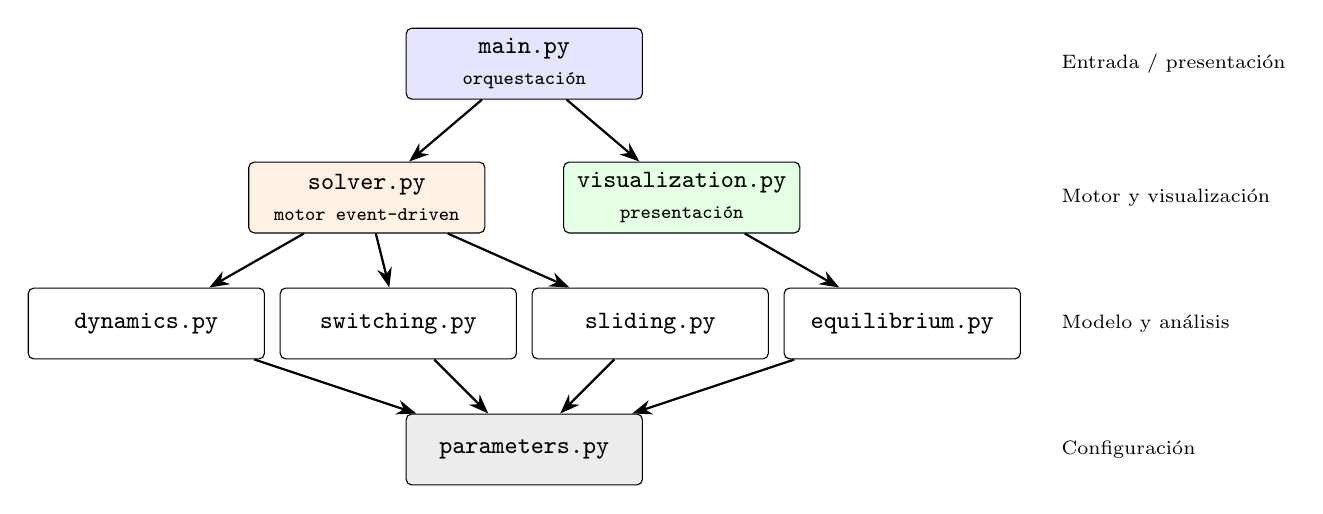
\begin{tikzpicture}[
  box/.style={draw, rounded corners=2pt, rectangle, align=center, font=\small\ttfamily, minimum width=3.0cm, minimum height=0.9cm},
  arr/.style={-{Stealth[length=2.5mm]}, thick},
  lbl/.style={font=\scriptsize, anchor=west}
]
  \node[box, fill=blue!10] (main) at (0,0) {main.py\\\scriptsize orquestación};
  \node[box, fill=orange!10] (solver) at (-2.0,-1.7) {solver.py\\\scriptsize motor event-driven};
  \node[box, fill=green!10] (vis) at (2.0,-1.7) {visualization.py\\\scriptsize presentación};
  \node[box] (dyn) at (-4.8,-3.3) {dynamics.py};
  \node[box] (swi) at (-1.6,-3.3) {switching.py};
  \node[box] (sld) at (1.6,-3.3) {sliding.py};
  \node[box] (eq) at (4.8,-3.3) {equilibrium.py};
  \node[box, fill=gray!15] (par) at (0,-4.9) {parameters.py};
  \node[lbl] at (6.7,0) {Entrada / presentación};
  \node[lbl] at (6.7,-1.7) {Motor y visualización};
  \node[lbl] at (6.7,-3.3) {Modelo y análisis};
  \node[lbl] at (6.7,-4.9) {Configuración};
  \draw[arr] (main) -- (solver);
  \draw[arr] (main) -- (vis);
  \draw[arr] (solver) -- (dyn);
  \draw[arr] (solver) -- (swi);
  \draw[arr] (solver) -- (sld);
  \draw[arr] (vis) -- (eq);
  \draw[arr] (dyn) -- (par);
  \draw[arr] (swi) -- (par);
  \draw[arr] (sld) -- (par);
  \draw[arr] (eq) -- (par);
\end{tikzpicture}
\caption{Arquitectura modular por capas del algoritmo. Las dependencias fluyen hacia abajo desde el punto de entrada hasta la capa de configuración.}
\label{fig:capas}
\end{figure}

\subsection{Flujo general del bucle event-driven}
\label{sec:flujo}
El corazón del algoritmo es la función \texttt{solver.simulate()}, cuya lógica reproduce el Algoritmo 1 de \cite{piiroinen2008event}. El pseudocódigo completo se presenta en la Sección 3.8 y el diagrama de flujo en la Figura~\ref{fig:flujo}. El bucle principal se repite hasta alcanzar \texttt{max\_switches} conmutaciones:

\begin{enumerate}
    \item Determinar la región actual ($y < w$: sistema 1; $y > w$: sistema 2; $y = w$: frontera).
    \item Integrar el campo vectorial correspondiente con \texttt{scipy.integrate.solve\_ivp} hasta que el evento $y(t) - w = 0$ (terminal) detenga la integración.
    \item Si no hubo evento, la trayectoria permaneció en su región y la simulación termina. En caso contrario, el último punto del arreglo de la solución es el punto de conmutación.
    \item Clasificar el punto de cruce mediante el criterio $L = f_{1y} \cdot f_{2y}$ y actuar según el tipo (cruce, deslizamiento o tangencia).
    \item Verificar que la trayectoria permanezca dentro del dominio $[a_x,b_x]\times[a_y,b_y]$; si sale, terminar.
\end{enumerate}

Cada tramo integrado se almacena en una estructura \texttt{TrajectorySegment} (coordenadas, tipo de segmento) y la lista completa de segmentos, junto con los puntos de tangencia alcanzados y el punto final, se agrupa en un \texttt{SimulationResult}. De esta forma la simulación queda descompuesta en piezas reutilizables y trazables, en línea con los atributos de mantenibilidad discutidos en la Sección 2.2.

\subsection{Capa de configuración: \texttt{parameters.py}}
La base de la arquitectura (Figura~\ref{fig:capas}) centraliza toda la configuración en tres \emph{dataclasses} inmutables (\texttt{frozen=True}): \texttt{FilippovParams} define los parámetros del modelo ($R_0$, $\mu$, $\theta$, $u$, $w$); \texttt{DomainParams} fija los límites del plano de fase $[0,1]\times[0,1]$; y \texttt{SolverParams} reúne las opciones del integrador: \texttt{tiempo\_max}=50, \texttt{max\_switches}=8, \texttt{max\_step}=0.01, tolerancias \texttt{rtol}=$10^{-3}$ y \texttt{atol}=$10^{-6}$, la perturbación \texttt{eps}=$10^{-6}$ y la tolerancia \texttt{tol}=$10^{-8}$. La inmutabilidad impide cambios accidentales y la inyección tipada de estos objetos como argumentos elimina las variables globales dispersas.

\subsection{Modelado de la dinámica: \texttt{dynamics.py}}
La capa de modelado define los dos campos vectoriales y el campo de deslizamiento. Al identificarse $\dot{x}$ con la población susceptible, se tiene \texttt{vector\_field\_1} (sistema 1, sin control):
\begin{equation}
f_1(\mathbf{x}) = \begin{pmatrix} \mu(1-x) - (\mu+\theta)R_0\,x\,y \\ (\mu+\theta)\,y\,(R_0 x - 1) \end{pmatrix},
\end{equation}
y \texttt{vector\_field\_2} (sistema 2, con control $u$):
\begin{equation}
f_2(\mathbf{x}) = \begin{pmatrix} \mu(1-x) - (\mu+\theta)R_0\,x\,y \\ (\mu+\theta)\,y\,(R_0 x - 1) - u \end{pmatrix}.
\end{equation}
El punto clave es que \textbf{la componente $x$ es idéntica en ambos sistemas} ($f_{1x} \equiv f_{2x}$); solo difiere la componente vertical por el término $-u$. Por ello, la dinámica de deslizamiento sobre $\Sigma$ ($y = w$) se reduce a la ODE unidimensional \texttt{sliding\_field\_1d}:
\begin{equation}
\dot{x} = \mu(1-x) - (\mu+\theta)R_0\,x\,w .
\end{equation}

\subsection{Análisis geométrico del plano de fase}
Los módulos \texttt{equilibrium.py} y \texttt{switching.py} precalculan la información geométrica que orienta la simulación.

\textbf{Puntos de equilibrio.} Para el sistema 1, el equilibrio endémico es $(S^*, I^*) = (1/R_0,\, \mu(R_0-1)/((\mu+\theta)R_0))$. Para el sistema 2, la condición $\dot{y}=0$ conduce a la ecuación cuadrática $\mu R_0 x^2 - (\mu + \mu R_0 - u R_0)x + \mu = 0$; si su discriminante es negativo no existen equilibrios reales y \texttt{compute\_equilibria} devuelve \texttt{NaN}.

\textbf{Puntos tangentes.} Un campo es tangente a $\Sigma$ cuando su proyección vertical se anula ($f_{iy}=0$):
\begin{equation}
T_1 = \left(\frac{1}{R_0}, w\right), \qquad
T_2 = \left(\frac{1}{R_0}\left(1 + \frac{u}{(\mu+\theta)\,w}\right), w\right) .
\end{equation}
Entre $T_1$ y $T_2$ se encuentra la zona de deslizamiento, donde los campos apuntan en direcciones opuestas.

\textbf{Criterio de conmutación.} Con $h = y - w$, la proyección de cada campo sobre $\nabla h$ es su componente vertical, por lo que el producto $L = f_{1y}(x,w)\cdot f_{2y}(x,w)$ clasifica el comportamiento en $\Sigma$ \cite{piiroinen2008event}: si $L>0$ ambos campos apuntan al mismo lado (\texttt{CROSSING}); si $L<0$ apuntan en direcciones opuestas (\texttt{SLIDING}); si $L\approx 0$ al menos un campo es tangente (\texttt{TANGENCY}). La enumeración \texttt{SwitchType} y la \emph{dataclass} \texttt{SwitchAnalysis} ($L$, $f_{1y}$, $f_{2y}$, tipo) encapsulan esta clasificación tipo-segura.

\textbf{Formulación clásica de Filippov.} El deslizamiento admite una descripción equivalente mediante la combinación convexa que anula la proyección vertical sobre $\Sigma$:
\begin{equation}
f_F(\mathbf{x}) = (1-\beta)\, f_1(\mathbf{x}) + \beta\, f_2(\mathbf{x}), \qquad
\beta = \frac{f_{1y}}{f_{1y} - f_{2y}} ,
\end{equation}
denominada convexificación de Filippov \cite{filippov1988}. Como $f_{1x}\equiv f_{2x}$, la componente horizontal de $f_F$ no depende de $\beta$ y coincide con la ODE unidimensional (3); por ello $\texttt{sliding\_field\_1d}$ implementa exactamente el campo de Filippov restringido a $\Sigma$. La condición de deslizamiento $\beta\in[0,1]$ es equivalente al criterio $L<0$: $\beta\in(0,1)$ se cumple si y solo si $f_{1y}$ y $f_{2y}$ tienen signos opuestos (es decir $L<0$), y los extremos $\beta=0$ y $\beta=1$ corresponden a las tangencias en $T_1$ y $T_2$ ($L=0$).

\subsection{Integración numérica y detección de cruces}
La capa \texttt{solver.py} construye, mediante la fábrica \texttt{make\_crossing\_event}, la función de evento $g(t) = y(t) - w$ con \texttt{terminal=True} y \texttt{direction}=$+1$ (si parte de la región inferior) o $-1$ (si parte de la superior). \texttt{solve\_ivp} detecta el cambio de signo de $g(t)$ entre pasos consecutivos y localiza el instante de impacto $t^*$ con $g(t^*)=0$ resolviendo la raíz dentro del intervalo de integración: el refinamiento de scipy interpola el polinomio asociado al esquema de Runge--Kutta interno, lo que es conceptualmente equivalente a un método de búsqueda de raíces (bisección/Brent) con la ventaja de ser consistente con el orden del integrador. De este modo, el último punto de la solución coincide con la intersección con $\Sigma$, $x(t^*)$, salvo la tolerancia del integrador. La trayectoria se mantiene suficientemente fina mediante \texttt{max\_step}=0.01 para evitar saltar la frontera entre pasos.

Cuando \texttt{compute\_switching\_analysis} clasifica el cruce:
\begin{itemize}
    \item \textbf{CROSSING}: se empuja la trayectoria al otro lado con la perturbación infinitesimal $y \leftarrow w \pm \varepsilon$, $\varepsilon=10^{-6}$, garantizando que el siguiente paso parta de la región correcta.
    \item \textbf{SLIDING}: se invoca la integración de deslizamiento de la Sección 3.6.
    \item \textbf{TANGENCY}: se registra el punto en \texttt{tangent\_hits} y se decide el lado de salida según el signo de la componente vertical del campo no tangente.
\end{itemize}
Si la trayectoria cae \emph{exactamente} sobre la frontera al inicio de una iteración, se aplica el mismo procedimiento de clasificación y posteriormente se ejecuta \texttt{continue}, evitando reintentar la integración desde $y = w$ con un subsistema indeterminado.

\subsection{Dinámica de deslizamiento: \texttt{sliding.py}}
Bajo la clasificación \texttt{SLIDING}, la función \texttt{integrate\_sliding} integra la ODE unidimensional (3) sobre $\Sigma$ con dos eventos terminales adicionales que detectan la llegada a $T_1$ (evento $x - x_{T_1} = 0$) y a $T_2$ (evento $x - x_{T_2} = 0$), con dirección 0 (cualquier sentido de cruce). Los indicadores \texttt{reached\_T1} y \texttt{reached\_T2} se leen de \texttt{sol.t\_events[0]} y \texttt{sol.t\_events[1]}, respectivamente, y la coordenada final del deslizamiento se toma de \texttt{sol.y\_events}. Al salir, se evalúa de nuevo $f_{1y}$: si es positiva la trayectoria escapa hacia arriba ($y = w + \varepsilon$) y si es negativa hacia abajo ($y = w - \varepsilon$). Este mecanismo implementa la salida del deslizamiento en los puntos tangentes, donde el parámetro de convexidad $\beta$ alcanza los extremos del intervalo $[0,1]$ ($\beta\notin(0,1)$) \cite{piiroinen2008event}.

\subsection{Orquestación y visualización}
\texttt{main.py} actúa como punto de entrada: instancia las tres \emph{dataclasses} de configuración, define las condiciones iniciales, ejecuta \texttt{simulate()} para cada una y delega el dibujo en \texttt{visualization.\allowbreak plot\_phase\_portrait()}. La capa de visualización evalúa los campos vectoriales sobre la cuadrícula de forma \textbf{vectorizada con \texttt{numpy}} (broadcasting matricial en lugar de bucles anidados, aproximadamente un orden de magnitud más rápido), dibuja la frontera con tres estilos (punteada fuera de $[T_1,T_2]$ y continua en la zona de deslizamiento) y superpone segmentos de trayectoria por tipo, equilibrios, puntos tangentes y condiciones iniciales.

\subsection{Detalles computacionales y pseudocódigo}
Desde el punto de vista computacional, el algoritmo alterna integraciones suaves de alto orden (\texttt{solve\_ivp} con control de tolerancia \texttt{rtol}/\texttt{atol}) con la resolución de raíces de eventos. La detección de eventos evita el \emph{chattering} de los métodos de paso fijo y mantiene el número de evaluaciones de función acotado.

En cuanto al uso de las estructuras de datos, todo el cálculo descansa en arreglos \texttt{numpy}: el integrador representa el estado como \texttt{V = [x, y]} y los campos vectoriales de \texttt{dynamics.py} reciben ese arreglo y lo procesan con operaciones vectoriales (\texttt{np.sqrt}, diferencias, productos entre escalares del mismo tipo), de modo que no hay conversiones intermedias tipo Python--NumPy ni bucles explícitos en el punto caliente del cómputo; la única conversión a listas ocurre al momento de \emph{almacenar} los segmentos ya integrados en \texttt{TrajectorySegment}. Esta elección evita el costo de interpretación de Python en cada evaluación de función y aprovecha el \emph{unboxing} que \texttt{solve\_ivp} utiliza internamente en sus etapas de Runge--Kutta. En la capa de visualización, además, los campos se evalúan sobre la cuadrícula completa con \emph{broadcasting} de \texttt{numpy} (operaciones matriciales en lugar de bucles anidados), aproximadamente un orden de magnitud más rápido que la evaluación punto a punto.

La integración con \texttt{scipy.integrate.solve\_ivp} aporta dos ventajas numéricas centrales al esquema event-driven. Primero, el paso de integración es \emph{adaptativo}: el tamaño del paso se ajusta en cada etapa para satisfacer el criterio $\lvert \text{error} \rvert \leq \mathit{atol} + \mathit{rtol}\,\lvert y \rvert$, concentrando evaluaciones donde la solución varía rápido y alargando los pasos en las regiones suaves, lo que equilibra precisión y costo. Segundo, la localización del evento $g(t) = y(t)-w$ no depende del refinamiento del paso sino de la búsqueda de raíz del polinomio interpolante del esquema interno, lo que produce el instante de impacto $t^*$ con precisión consistente con el orden del integrador y mantiene el número de llamadas a la función acotado e independiente de la suavidad de la frontera. El pseudocódigo del bucle completo se muestra en el Algoritmo~\ref{alg:event-driven} y el diagrama de flujo en la Figura~\ref{fig:flujo} (los detalles numéricos de costo y precisión se evalúan en la Sección 4).

\begin{algorithm}[H]
\caption{Bucle event-driven de Filippov (adaptado de \cite{piiroinen2008event}, Algoritmo 1)}
\label{alg:event-driven}
\footnotesize
\begin{algorithmic}[1]
\State \textbf{Entrada:} $(x_0, y_0)$, $\mathit{fp}$, $\mathit{dp}$, $\mathit{sp}$
\State $x, y \gets x_0, y_0$; \ $n \gets 0$; \ $\mathit{result} \gets \text{SimulationResult}(x_0,y_0)$
\While{$n < \mathit{sp}.\text{max\_switches}$}
  \If{$y < w$}
    \State $\mathit{vf} \gets f_1$; \ $\mathit{tipo} \gets \text{sistema1}$
  \ElsIf{$y > w$}
    \State $\mathit{vf} \gets f_2$; \ $\mathit{tipo} \gets \text{sistema2}$
  \Else
    \State $a \gets \text{compute\_switching\_analysis}(x, w)$ \Comment{criterio $L = f_{1y}\,f_{2y}$}
    \If{$a = \text{SLIDING}$}
      \State $\mathit{slide} \gets \text{integrate\_sliding}(x, w, T_1, T_2)$
      \State $x \gets \mathit{slide}.x_{\mathrm{fin}}$; \ $y \gets w + \varepsilon$ si $f_{1y} > 0$, si no $w - \varepsilon$
    \ElsIf{$a = \text{TANGENCY}$}
      \State registrar tangencia; $y \gets w \pm \varepsilon$ (signo del campo no tangente)
    \Else
      \State $y \gets w \pm \varepsilon$ \Comment{cruce en la frontera}
    \EndIf
    \State \textbf{continue}
  \EndIf
  \State $\mathit{event} \gets$ cruce terminal $y(t) - w = 0$, dirección $\pm 1$
  \State $\mathit{sol} \gets \text{solve\_ivp}(\mathit{vf}, [0, t_{\max}], [x, y], \text{events}=\mathit{event})$
  \State guardar segmento $(\mathit{sol}.y, \mathit{tipo})$
  \If{no hubo evento} \State \textbf{break} \EndIf
  \State $(x, y) \gets$ último punto de $\mathit{sol}$ \Comment{punto de cruce en $\Sigma$}
  \State $a \gets \text{compute\_switching\_analysis}(x, w)$
  \If{$a = \text{CROSSING}$}
    \State $y \gets w + \varepsilon$ si $\mathit{tipo} = \text{sistema1}$, si no $y \gets w - \varepsilon$
  \ElsIf{$a = \text{SLIDING}$}
    \State $\mathit{slide} \gets \text{integrate\_sliding}(x, w, T_1, T_2)$
    \State guardar segmento sliding; $x \gets \mathit{slide}.x_{\mathrm{fin}}$
    \State $y \gets w + \varepsilon$ si $f_{1y} > 0$, si no $w - \varepsilon$
  \Else
    \State registrar tangencia; $y \gets w \pm \varepsilon$ (signo del otro campo)
  \EndIf
  \State $n \gets n + 1$
  \If{$(x, y)$ fuera de $\mathit{dp}$} \State \textbf{break} \EndIf
\EndWhile
\Statex
\State $\mathit{result}.\text{final\_point} \gets (x, y)$; \Return $\mathit{result}$
\end{algorithmic}
\end{algorithm}

\begin{figure}[H]
\centering
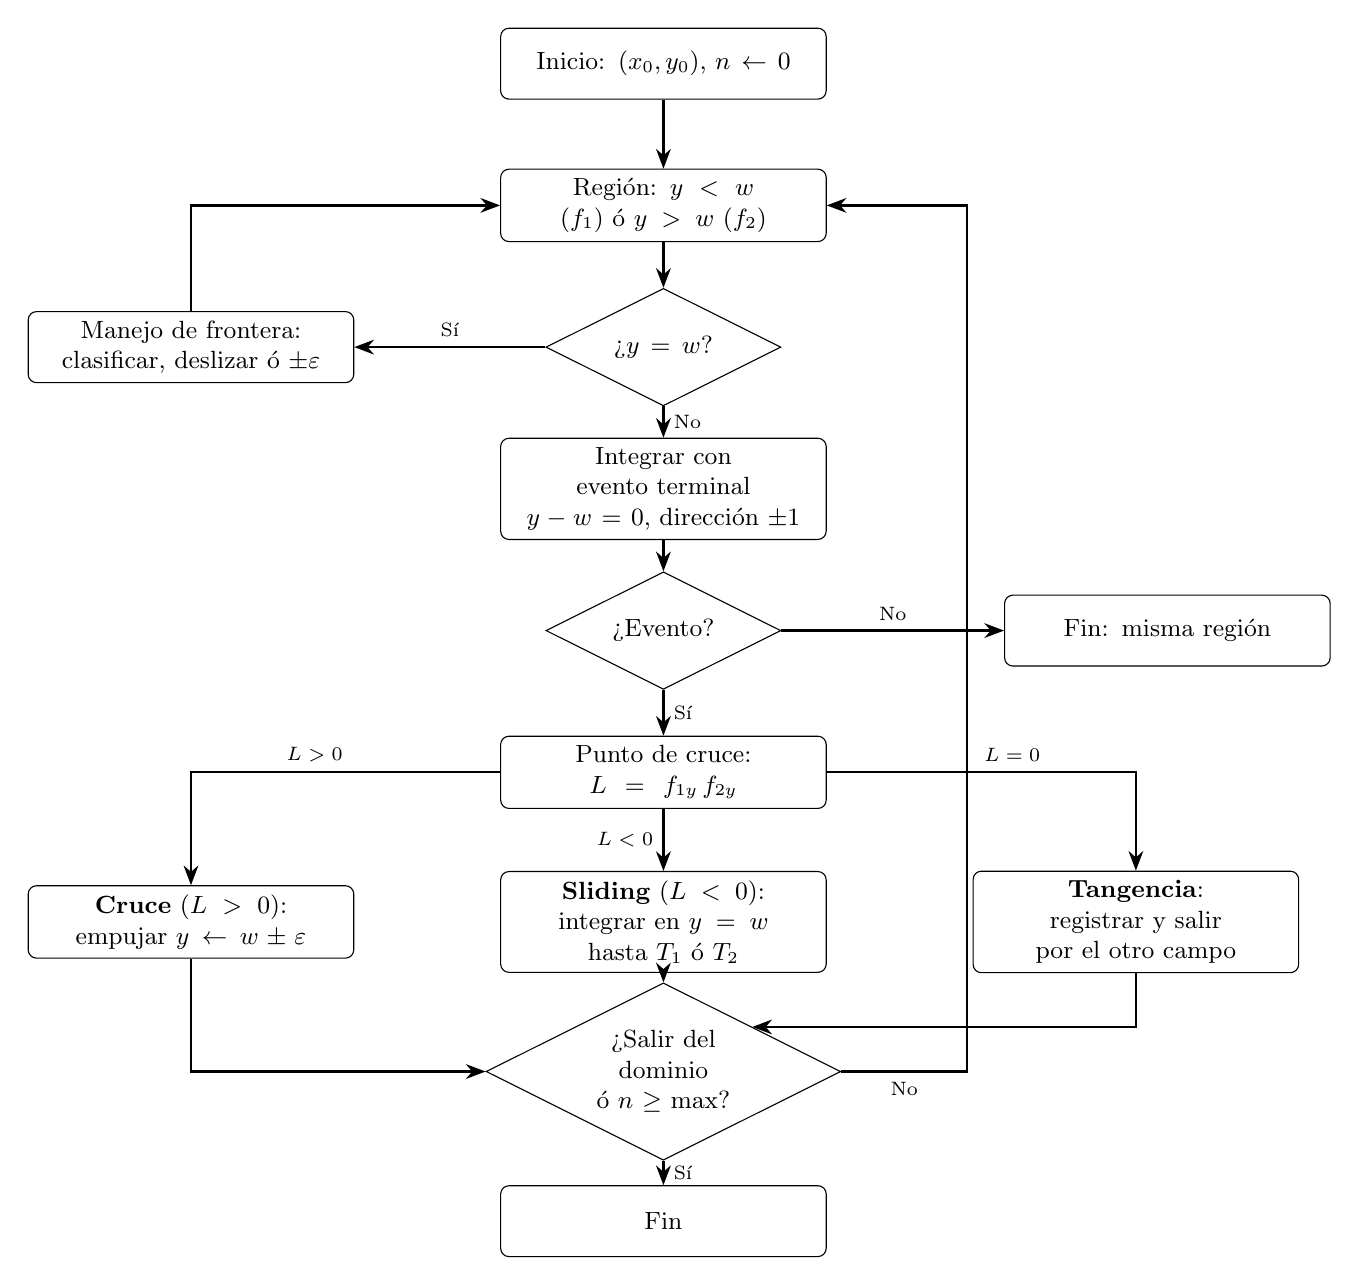
\begin{tikzpicture}[
  p/.style={rectangle, draw, rounded corners=3pt, align=center, text width=3.9cm, minimum height=0.9cm, font=\small},
  d/.style={diamond, draw, align=center, text width=2.0cm, inner sep=2pt, font=\small, aspect=2},
  arr/.style={-{Stealth[length=2.5mm]}, thick},
  lab/.style={font=\scriptsize}
]
  \node[p] (init) at (0,0) {Inicio: $(x_0, y_0)$, $n \gets 0$};
  \node[p] (reg) at (0,-1.8) {Región: $y<w$ ($f_1$) ó $y>w$ ($f_2$)};
  \node[d] (bnd) at (0,-3.6) {¿$y=w$?};
  \node[p] (bproc) at (-6.0,-3.6) {Manejo de frontera:\\clasificar, deslizar ó $\pm\varepsilon$};
  \node[p] (inte) at (0,-5.4) {Integrar con evento terminal\\$y-w=0$, dirección $\pm 1$};
  \node[d] (evh) at (0,-7.2) {¿Evento?};
  \node[p] (finc) at (6.4,-7.2) {Fin: misma región};
  \node[p] (clas) at (0,-9.0) {Punto de cruce:\\$L = f_{1y}\,f_{2y}$};
  \node[p] (cr) at (-6.0,-10.9) {\textbf{Cruce} ($L>0$):\\empujar $y \leftarrow w \pm \varepsilon$};
  \node[p] (sl) at (0,-10.9) {\textbf{Sliding} ($L<0$):\\integrar en $y=w$ hasta $T_1$ ó $T_2$};
  \node[p] (tn) at (6.0,-10.9) {\textbf{Tangencia}:\\registrar y salir por el otro campo};
  \node[d] (chk) at (0,-12.8) {¿Salir del dominio\\ó $n\ge$ max?};
  \node[p] (fin) at (0,-14.7) {Fin};
  \draw[arr] (init.south) -- (reg.north);
  \draw[arr] (reg.south) -- (bnd.north);
  \draw[arr] (bnd.west) -- node[lab,above]{Sí} (bproc.east);
  \draw[arr] (bnd.south) -- node[lab,right]{No} (inte.north);
  \draw[arr] (inte.south) -- (evh.north);
  \draw[arr] (evh.east) -- node[lab,above]{No} (finc.west);
  \draw[arr] (evh.south) -- node[lab,right]{Sí} (clas.north);
  \draw[arr] (clas.west) -| node[lab,above,pos=0.3]{$L>0$} (cr.north);
  \draw[arr] (clas.south) -- node[lab,left]{$L<0$} (sl.north);
  \draw[arr] (clas.east) -| node[lab,above,pos=0.3]{$L=0$} (tn.north);
  \draw[arr] (cr.south) |- (chk.west);
  \draw[arr] (sl.south) -- (chk.north);
  \draw[arr] (tn.south) |- (chk.north east);
  \draw[arr] (bproc.north) |- (reg.west);
  \draw[arr] (chk.south) -- node[lab,right]{Sí} (fin.north);
  \draw[arr] (chk.east) -- node[lab,below]{No} ++(1.6,0) |- (reg.east);
\end{tikzpicture}
\caption{Diagrama de flujo del bucle event-driven implementado en \texttt{solver.simulate()}.}
\label{fig:flujo}
\end{figure}

\section{Casos de estudio y resultados numéricos}
Para presentar la implementación del algoritmo en los sistemas de Filippov, se presentarán 2 casos de estudio: un sistema en $\mathbb{R}^2$ y otro sistema en $\mathbb{R}^3$.
\subsection{Caso 1}
Se presenta el planteamiento y solución numérica del modelo Lokta-Volterra en $\mathbb{R}^2$ planteado en \cite{kuznetsov2003one}.
\subsection{Caso 2}
Presentación del planteamiento y análisis de un modelo tridimensional tipo Filippov.
\subsection{Métricas de evaluación del algoritmo}
\begin{itemize}
    \item Error cuadrático medio respecto a soluciones analíticas/de alta precisión.
    \item Tiempo de ejecución (CPU time) frente a solvers nativos de Python.
    \item Control del número de evaluaciones de función ($N_{eval}$).
\end{itemize}

\section{Conclusiones y Discusión}
Hablar sobre los resultados obtenidos y tropiesos que se tienen para llegar a las soluciones o mejorar el rendimiento del código, resaltando:
\begin{itemize}
    \item Ventajas operativas frente a métodos convencionales sin detección de eventos.
    \item Complejidad computacional e impacto en el desarrollo de software académico.
    \item Limitaciones del algoritmo (ej. superficies de conmutación múltiples o no diferenciables).
    \item Se tiene una dependencia de un estudio analítico previo.
\end{itemize}

% --- IMPRIMIR LA BIBLIOGRAFÍA ---
\printbibliography[title={Referencias}] 

\end{document}